% coding:utf-8

%----------------------------------------
%FOSAMATH, a LaTeX-Code for a mathematical summary for basic analysis
%Copyright (C) 2013, Daniel Winz, Ervin Mazlagic, Adrian Imboden, Philipp Langer

%This program is free software; you can redistribute it and/or
%modify it under the terms of the GNU General Public License
%as published by the Free Software Foundation; either version 2
%of the License, or (at your option) any later version.

%This program is distributed in the hope that it will be useful,
%but WITHOUT ANY WARRANTY; without even the implied warranty of
%MERCHANTABILITY or FITNESS FOR A PARTICULAR PURPOSE.  See the
%GNU General Public License for more details.
%----------------------------------------

% coding:utf-8

\section{Krümmung}

Die Krümmung $\kappa$ misst wie stark eine Kurve $\gamma$ gekrümmt ist (vgl. 
Kreis hat eine konstante Krümmung).
Die Krümmung wird unterschieden in mittlere und momentane Krümmung.
\begin{figure}[h!]
\centering
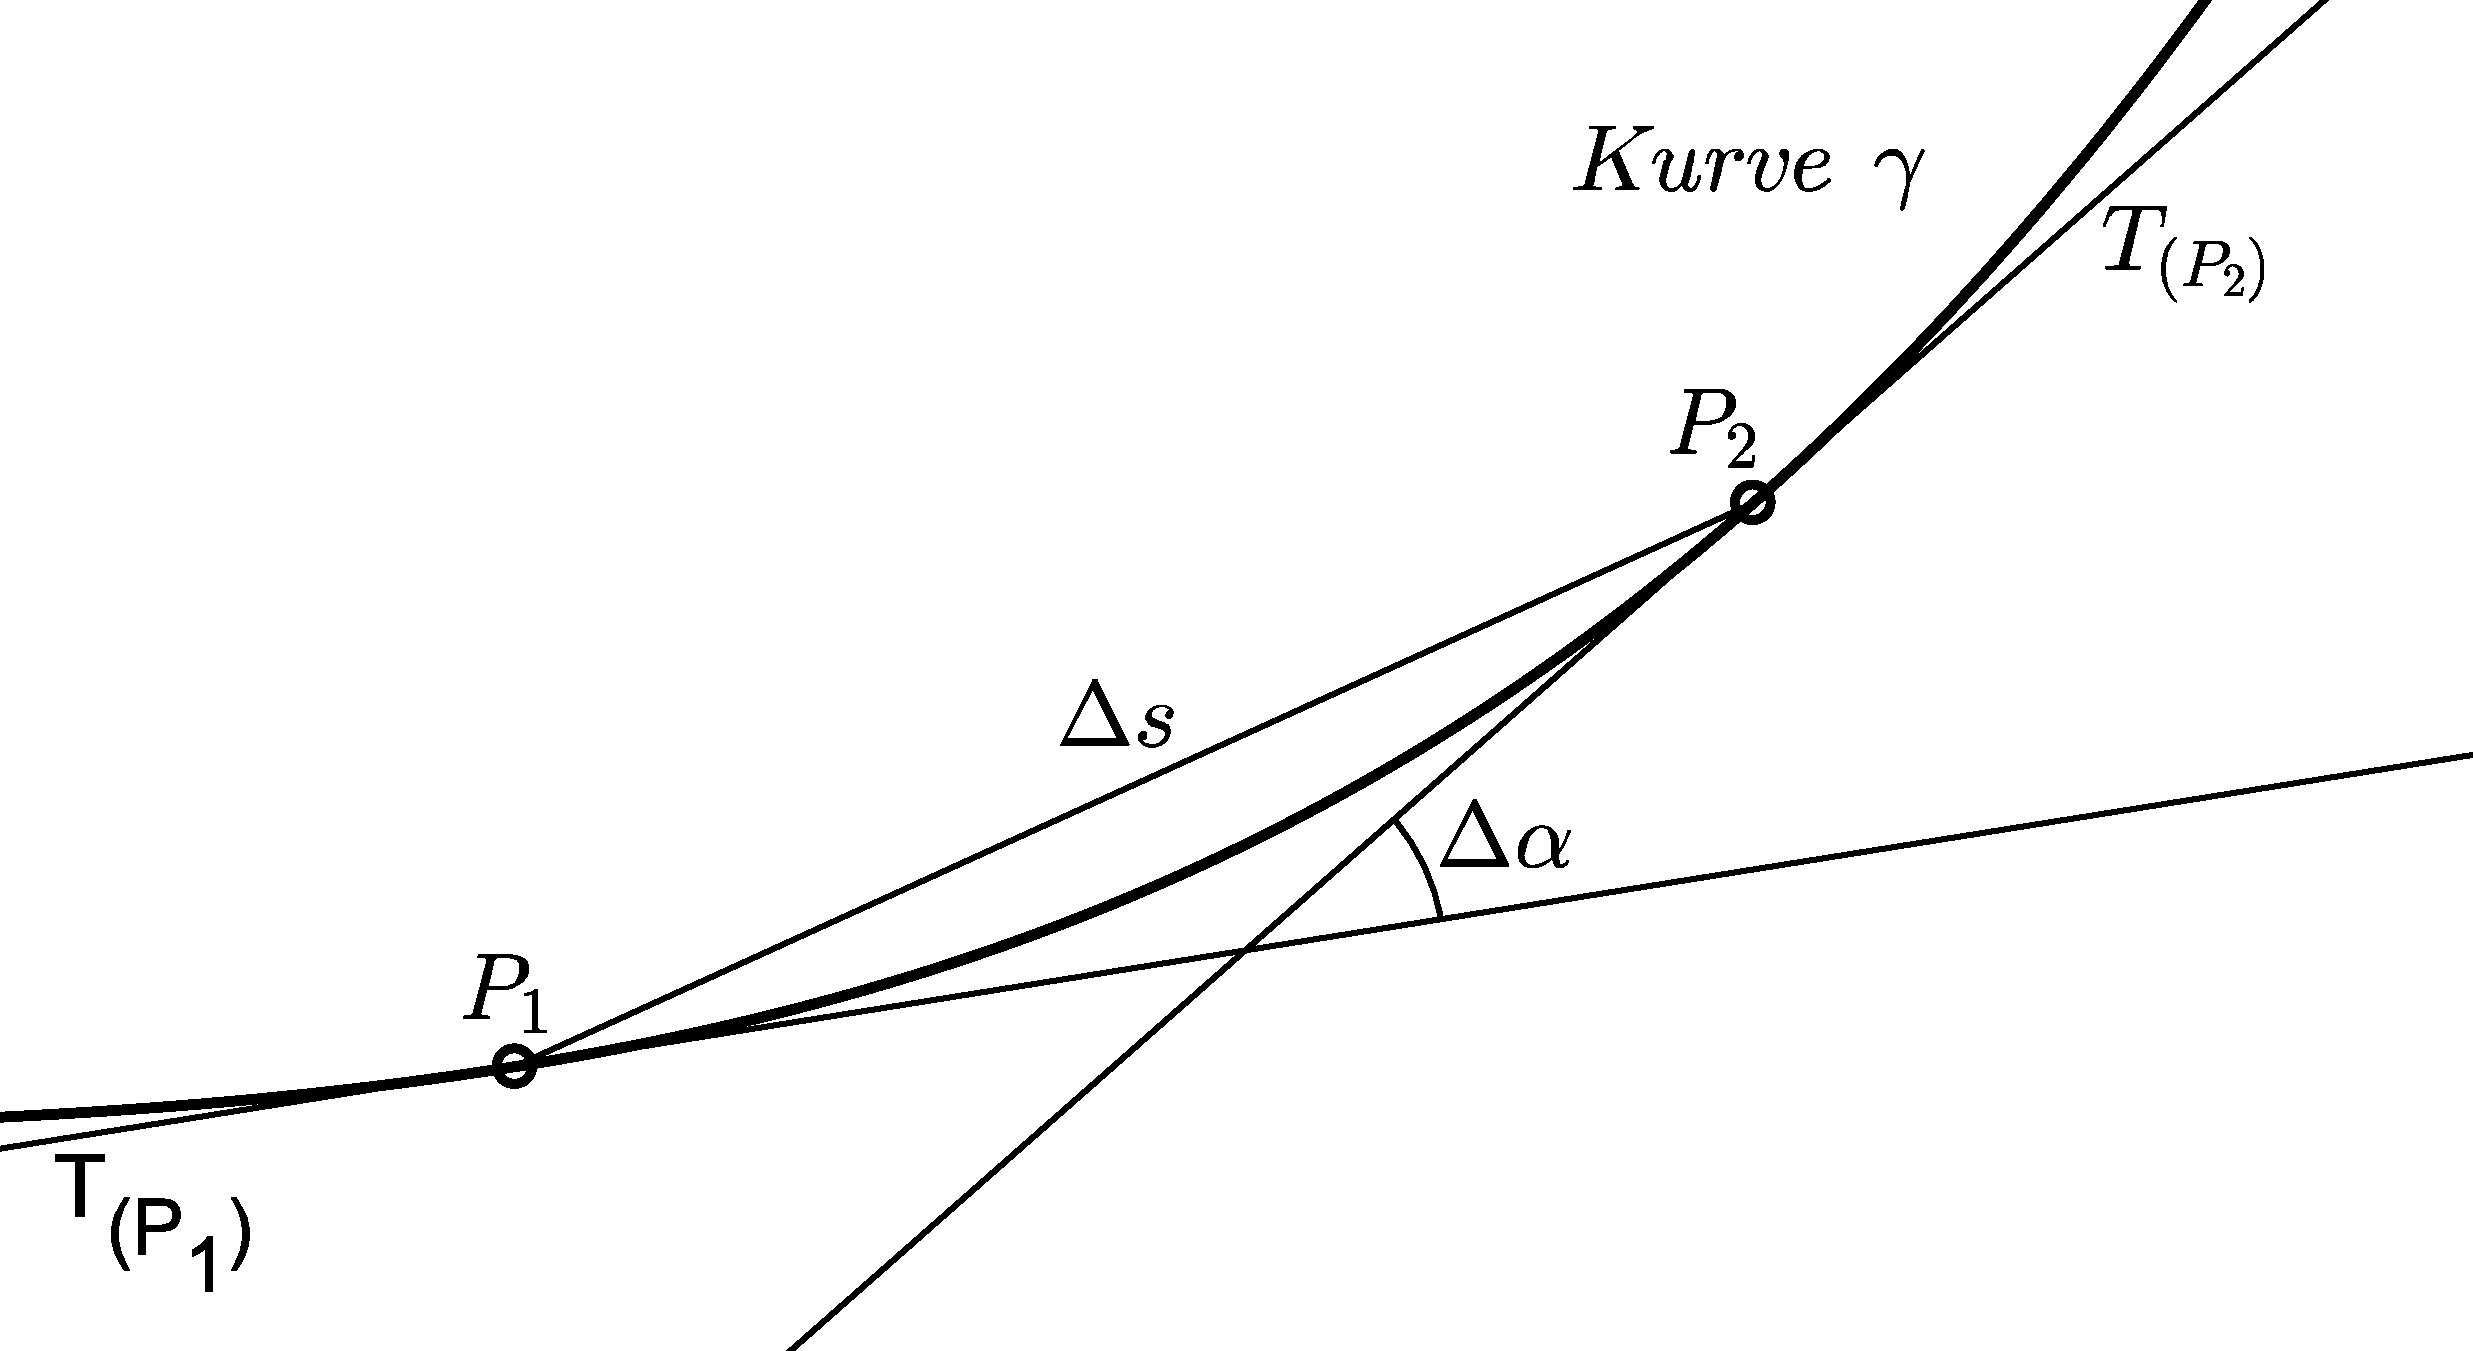
\includegraphics[width=0.8\textwidth]{kruemmung.pdf}
\end{figure}

\[ \begin{array}{ll}
	\text{mittlere}  & \dfrac{\Delta \alpha}{\Delta s} \\
	& \\
	\text{momentane} & \dfrac{\delta \alpha}{\delta s} \\
\end{array} \]

\begin{figure}[h!]
\centering
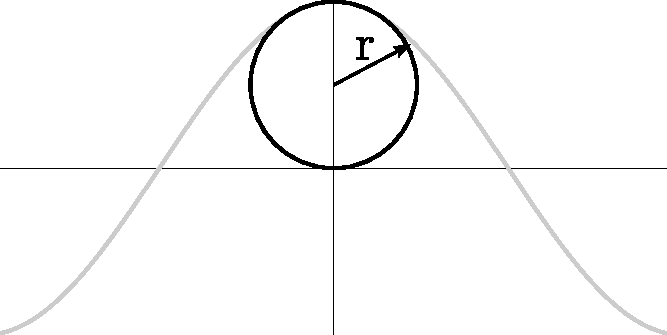
\includegraphics[width=0.5\textwidth]{kruemmungsradius.pdf}
\end{figure}
\[ \boxed{r(t) = \dfrac{1}{|\kappa(t)|} \quad \quad \text{bzw.} 
\quad \quad r(x) = \dfrac{1}{|\kappa(x)|} } \]
\[ \boxed{\kappa(x) = \frac{y''(x)}{(1 + y'(x)^2)^{\frac{3}{2}}} }\]

\[\boxed{\begin{array}{lllll} 
	\kappa (x) > 0 & \rightarrow & y''(x) \stackrel{!}{>} 0 
    & \xrightarrow[]{\phantom{Achtung!}} & y \text{ ist konvex} \\
	\kappa (x) < 0 & \rightarrow & y''(x) \stackrel{!}{<} 0 
    & \xrightarrow[]{\phantom{Achtung!}} & y \text{ ist konkav} \\
	\kappa (x) = 0 & \rightarrow & y''(x) = 0		
    & \xrightarrow[]{Achtung!} & \text{Wendepunkt!}
\end{array}}\]
\section{Scheitelpunkte}
Scheitelpunkte sind Stellen an denen die Krümmung maximal ist. 
Um diese zu berechnen muss die Krümmung $\kappa (x)$ abgeleitet und Null 
gesetzt werden.
\[ \kappa '(x) \stackrel{!}{=} 0  \]
\[ \boxed{\kappa '(x) = \dfrac{ y'''(x)(1+y'(x)^2)^{\frac{3}{2}} - y''(x) 
\frac{3}{2}(1+y'(x)^2)^{\frac{1}{2}} 2y''(x) }{ (1+y'(x)^2)^3 } 
\stackrel{!}{=} 0 } \]
